\documentclass[border=10pt]{standalone}
\usepackage{tikz}
\usepackage{amsmath}
\definecolor{myblue}{RGB}{38,84,160}
\begin{document}
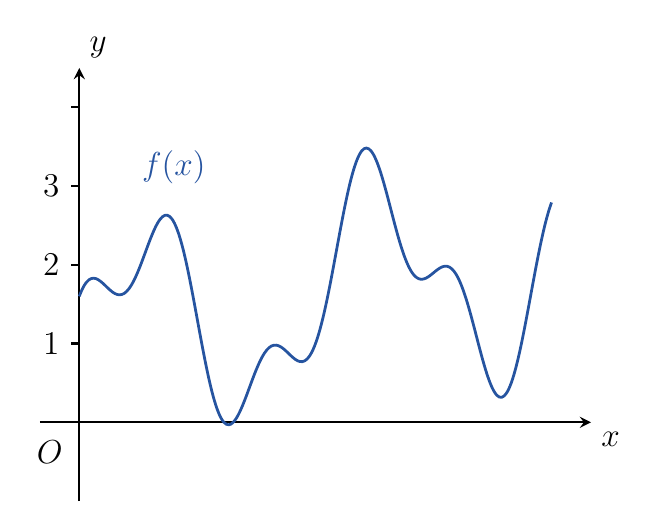
\begin{tikzpicture}[>=stealth, line width=0.8pt, font=\large,
    declare function={f(\x) = 1.2*sin(\x*120) + 0.6*cos(\x*300) + 0.2*\x + 1;}]

  % 坐标轴（同款风格）
  \draw[->] (-0.5,0) -- (6.5,0)   node[below right] {$x$};
  \draw[->] (0,-1.0) -- (0,4.5)   node[above right] {$y$};
  \coordinate (origin) at (0,0);
  % y 轴刻度
  \foreach \t in {1,2,3,4} \draw (0,\t) -- ++(-0.1,0);
  \foreach \t in {1,2,3}   \node[left] at (-0.12,\t) {$\t$};
  \node[below left] at (-0.08,-0.1) {$O$};

  % 目标函数曲线
  \draw[myblue, line width=1pt, smooth, samples=200, domain=0:6]
    plot (\x, {f(\x)});
  \node[myblue] at (1.2,{f(1.2)+0.7}) {$f(x)$};

\end{tikzpicture}
\end{document}